\lstinputlisting[language=bash,basicstyle=\small]{python_codes/fieldstone_16/keywords.ascii}

\begin{center}
Code at \url{https://github.com/cedrict/fieldstone/tree/master/python_codes/fieldstone_16}
\end{center}

\par\noindent\rule{\textwidth}{0.4pt}

%%%%%%%%%%%%%%%%%%%%%%%%%%%%%%%%%%%%%%%%%%%%%%%%%%%%%%%%%%%%%%%%%%%%%%%%%%%%%%%%%%%%%%%

We are revisiting the 2D Stokes sphere problem, but this time 
we use the Schur complement approach to solve the Stokes system. 
We choose an open boundary at the top so that we do not have to deal with the pressure 
nullspace. No-slip boundary conditions are prescribed on the sides and bottom boundaries.
Density and viscosity are prescribed directly onto the quadrature points. 

Because there are viscosity contrasts in the domain, it is advisable 
to use the Preconditioned Conjugate Gradient 
as presented in Section \ref{sec:solvers} (see {\bf solver\_pcg}).\\
The solver is implemented in the {\tt schur\_complement\_cg\_solver.py} file in the same folder.  

\begin{center} 
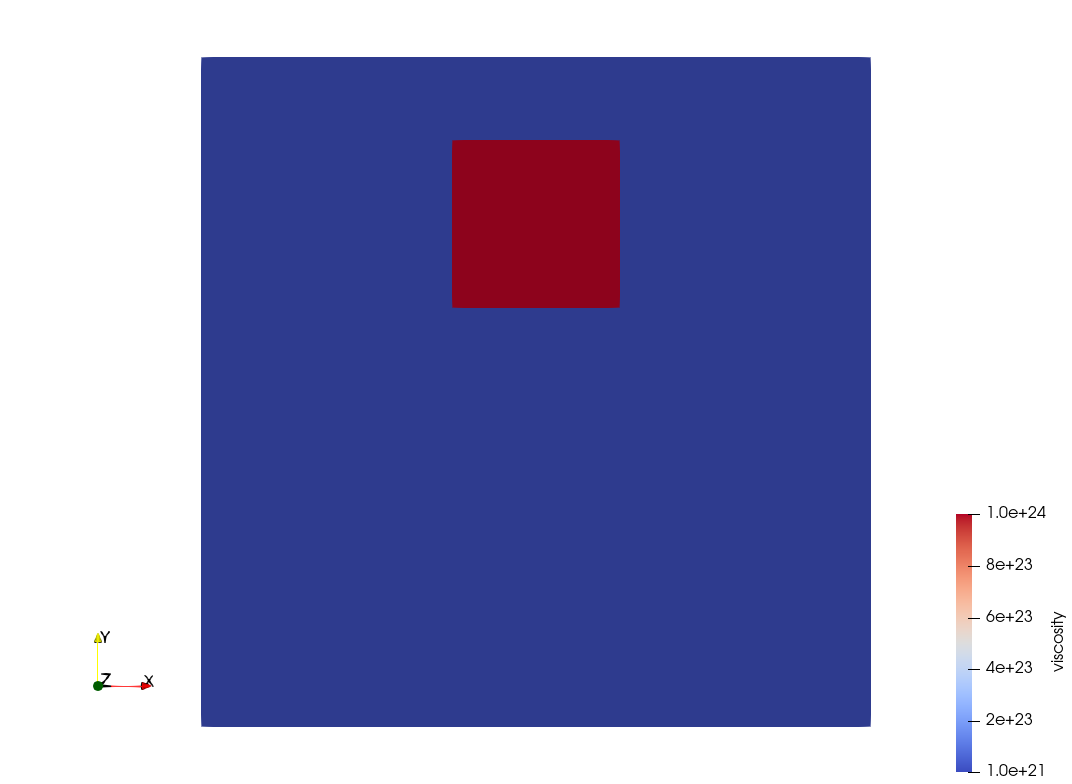
\includegraphics[width=5cm]{python_codes/fieldstone_16/results/eta}
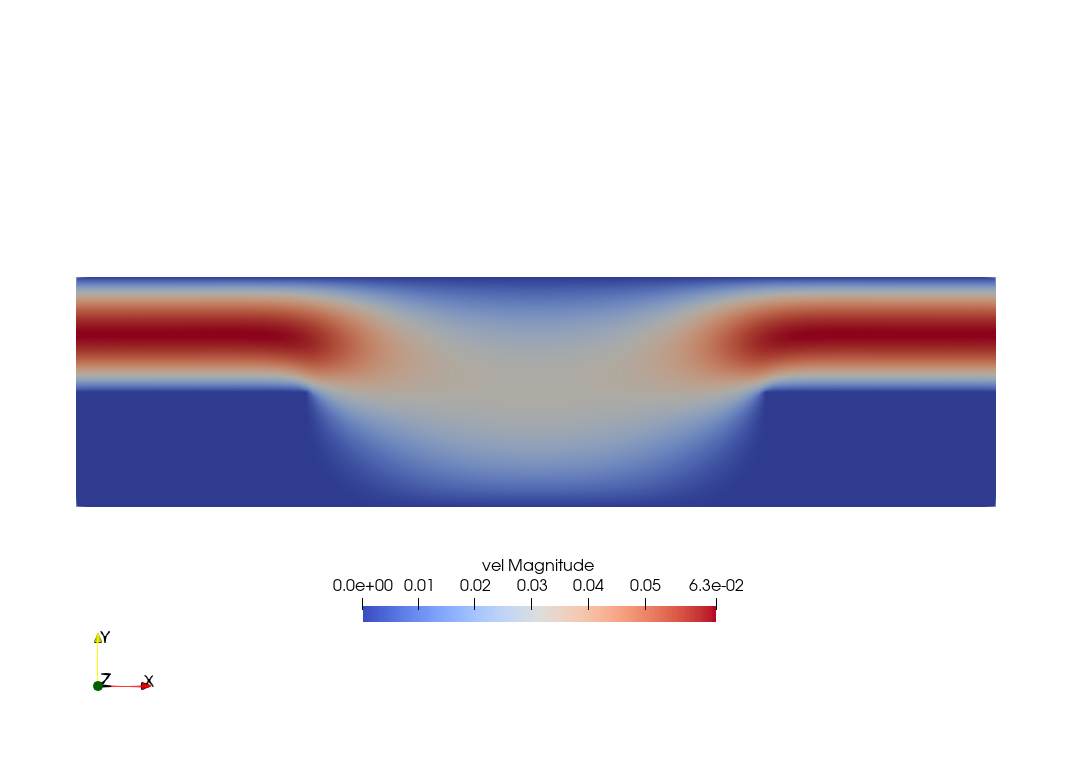
\includegraphics[width=5cm]{python_codes/fieldstone_16/results/vel}
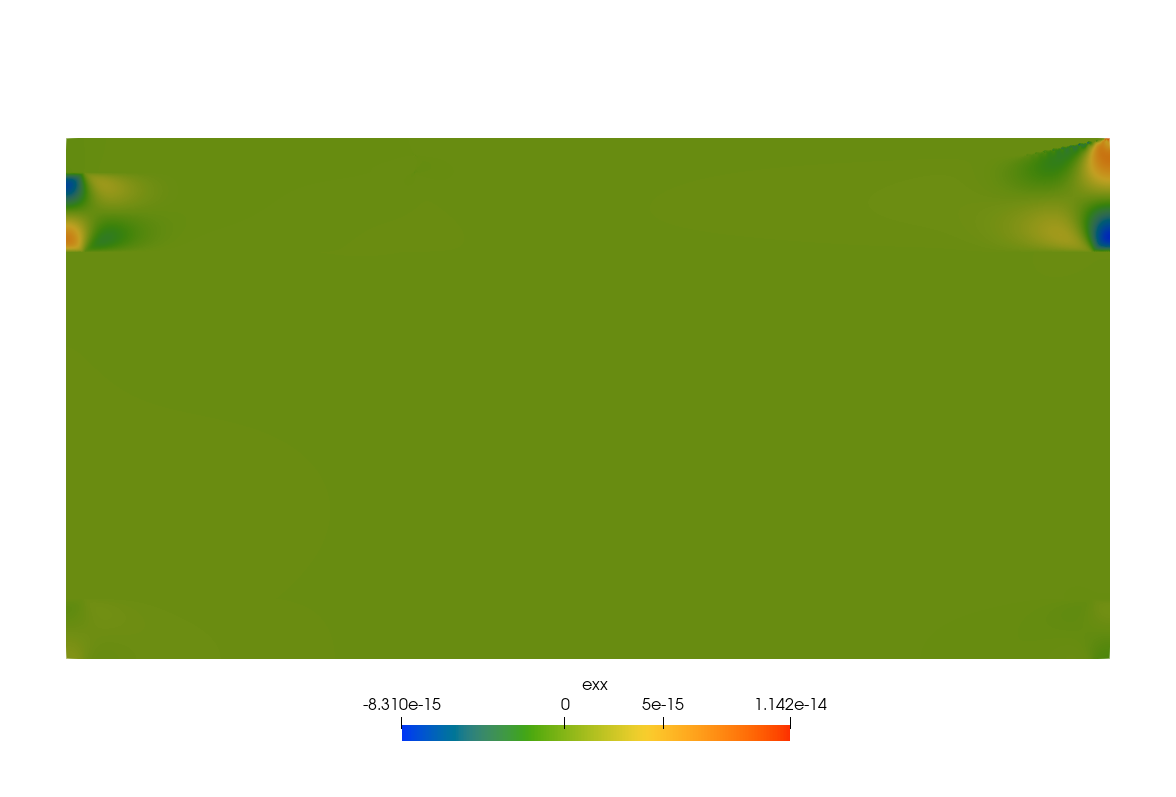
\includegraphics[width=5cm]{python_codes/fieldstone_16/results/exx}\\
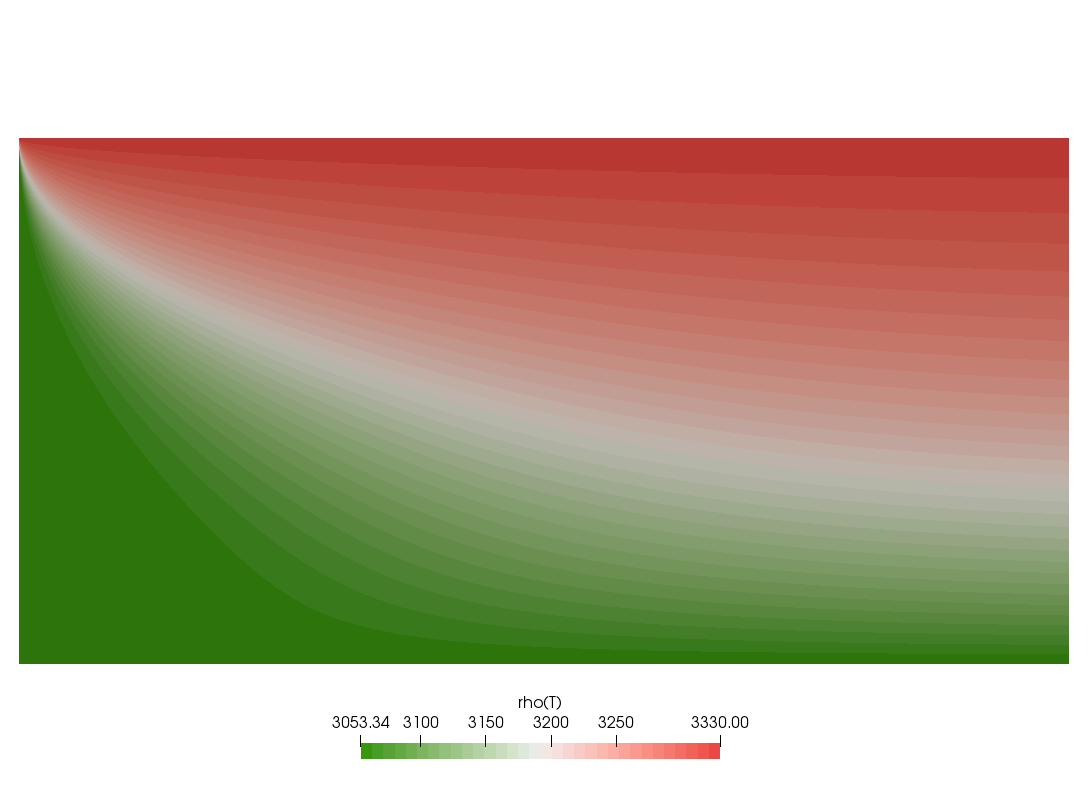
\includegraphics[width=5cm]{python_codes/fieldstone_16/results/rho}
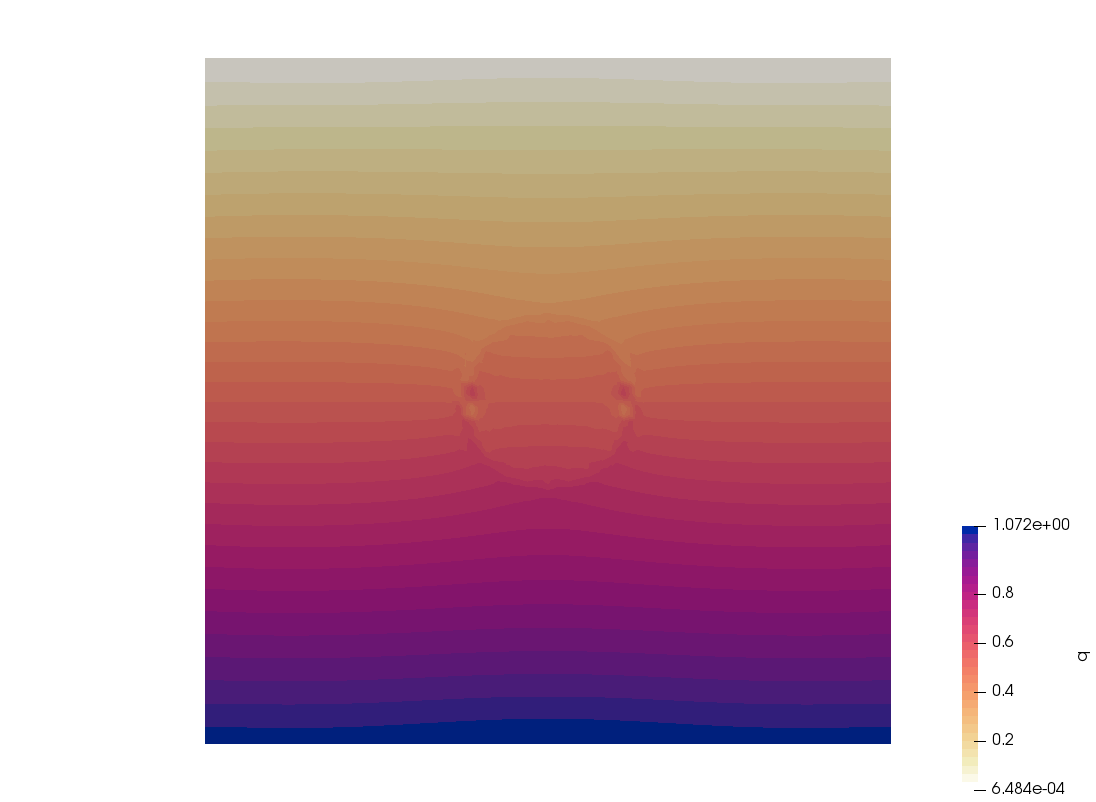
\includegraphics[width=5cm]{python_codes/fieldstone_16/results/q}
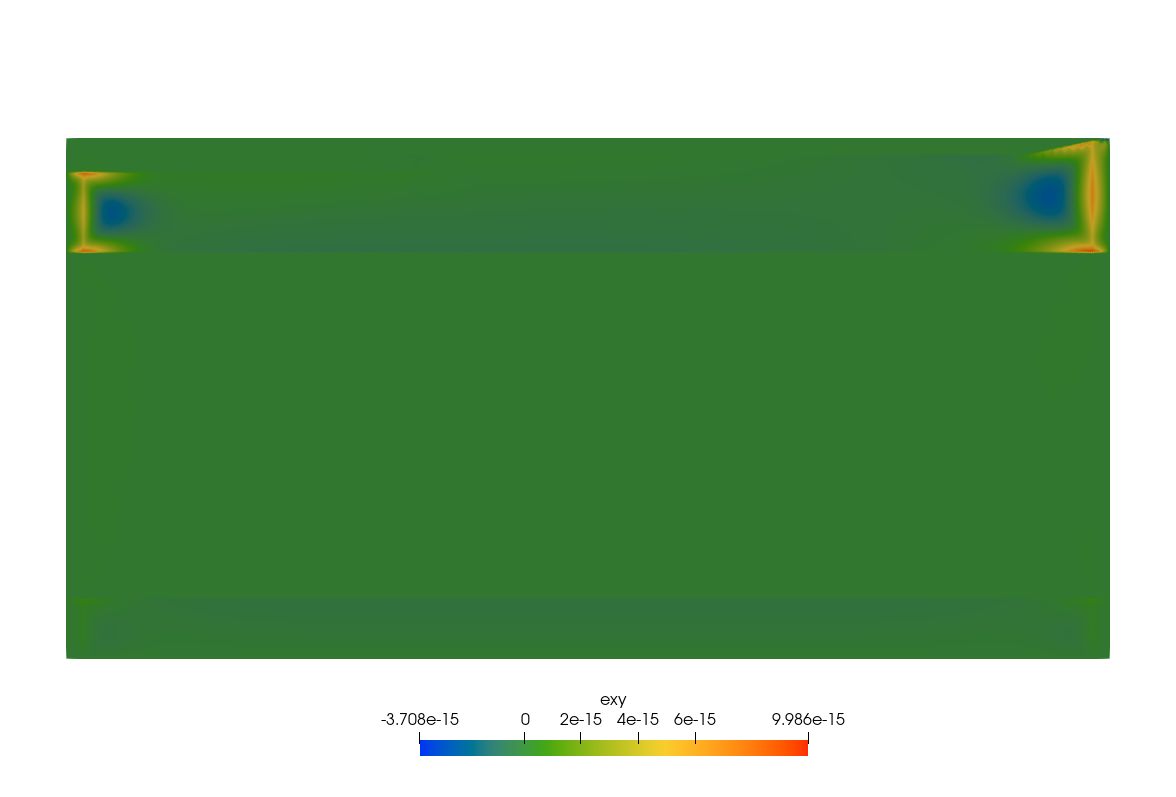
\includegraphics[width=5cm]{python_codes/fieldstone_16/results/exy}\\
{\captionfont Viscosity, density, velocity and pressure fields, resolution $96\times 96$.}
\end{center} 

We have designed 5 preconditioners:
\begin{itemize}
\item {\tt precond\_type=0} It is the unit matrix (so it does nothing). 
\item {\tt precond\_type=1} This is a very simple one as it is
diagonal and built element by element:
\[
M_{e,e} = \frac{h_x h_y}{\eta_e} 
\]
where $e$ is an element and $\eta_e$ the viscosity evaluated in its center. Note that 
averages based on quadrature point values could also be considered (or any other kind of projection).
\item {\tt precond\_type=2}
\[
{\bm M} = \G^T (diag [\K]  )^{-1} \G 
\]
\item {\tt precond\_type=3} 
\[
{\bm M} = diag \left[ \G^T (diag [\K]  )^{-1} \G \right]
\]
\item {\tt precond\_type=4} Same as 2, but instead of using the 
diagonal of $ \G^T (diag [\K]  )^{-1} \G$ we lump the matrix instead.

\end{itemize}


\begin{center} 
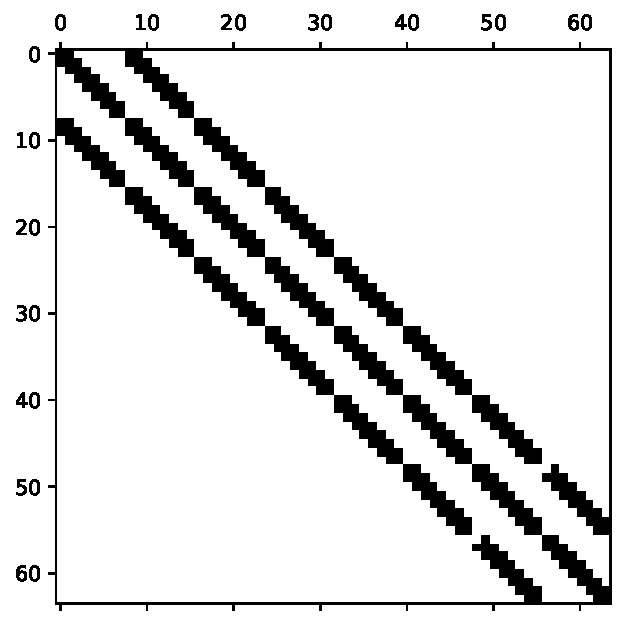
\includegraphics[width=5cm]{python_codes/fieldstone_16/results/matrix_ps2}
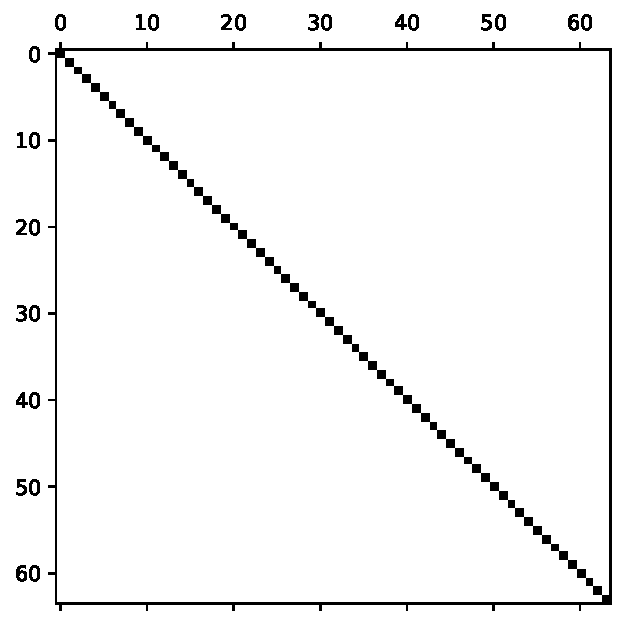
\includegraphics[width=5cm]{python_codes/fieldstone_16/results/matrix_ps3}\\
{\captionfont Resolution 8x8 elements. Matrix sparsity pattern 
for preconditioner \#2 (left) and preconditioners 0,1,3,4 (right).}
\end{center}


\begin{center} 
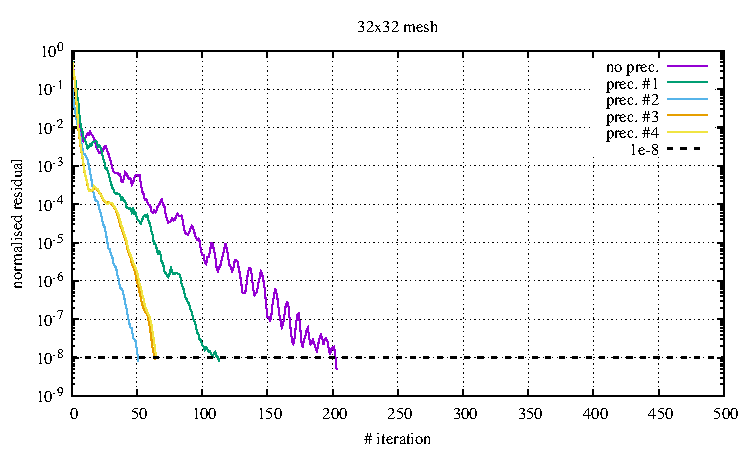
\includegraphics[width=5.4cm]{python_codes/fieldstone_16/results/residual_32x32.pdf}
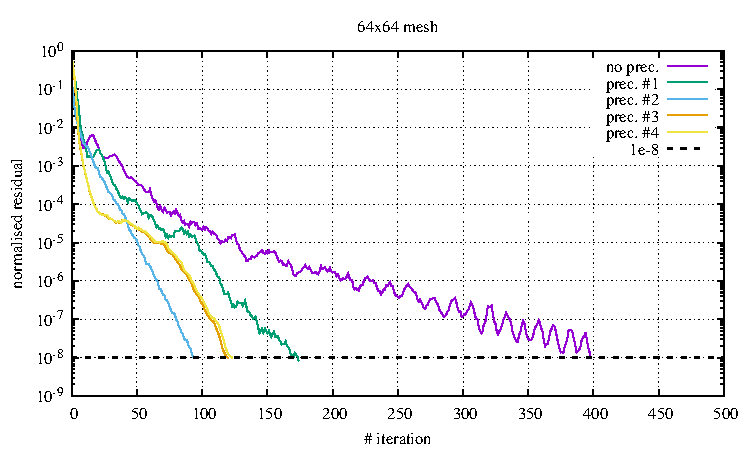
\includegraphics[width=5.4cm]{python_codes/fieldstone_16/results/residual_64x64.pdf}
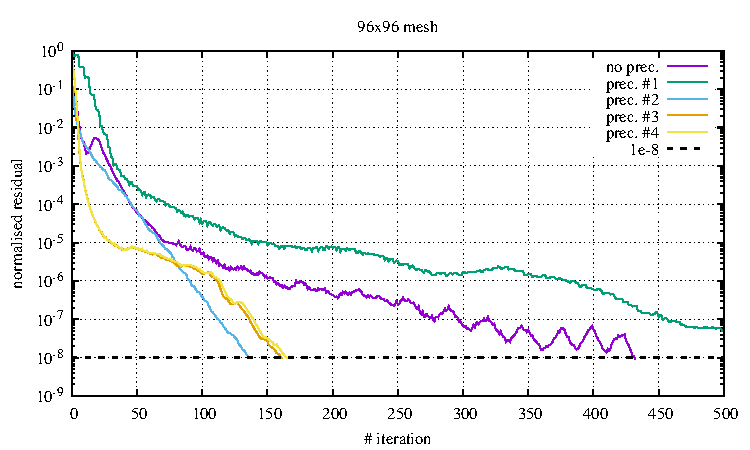
\includegraphics[width=5.4cm]{python_codes/fieldstone_16/results/residual_96x96.pdf}\\
{\captionfont Residual inside the solver as a function of the preconditioner type, 
and for two resolutions 32x32 (left), 64x64 (middle) and 96x96 (right).}
\end{center}


\begin{center} 
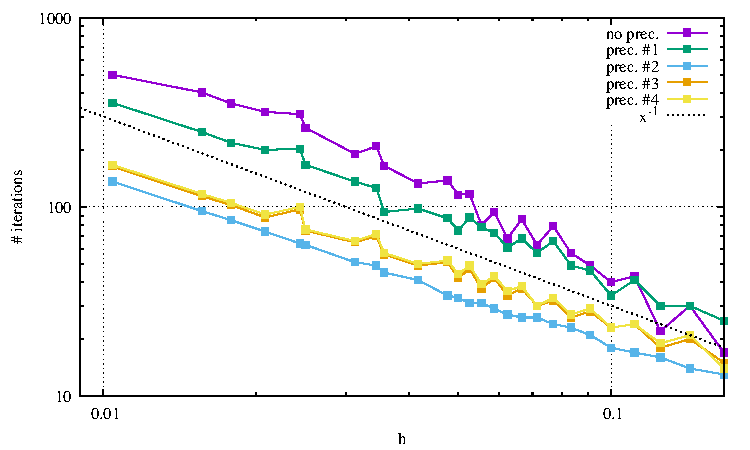
\includegraphics[width=5.4cm]{python_codes/fieldstone_16/results/niterations.pdf}
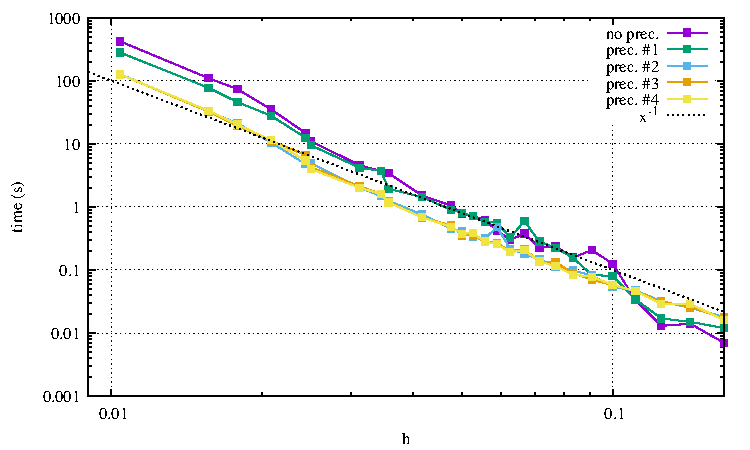
\includegraphics[width=5.4cm]{python_codes/fieldstone_16/results/solve_time.pdf}
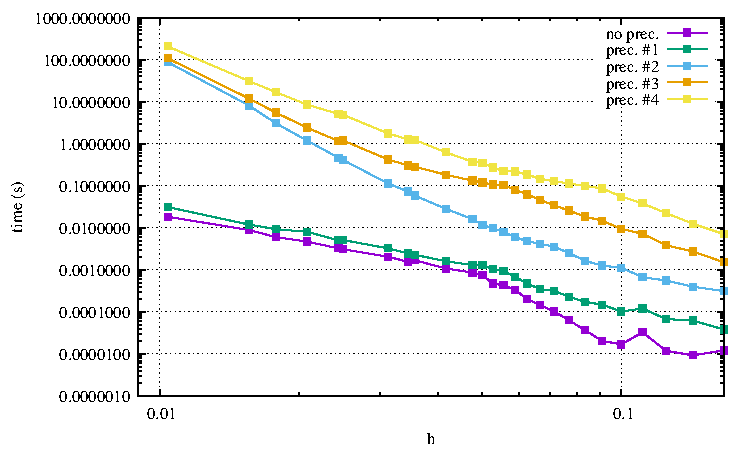
\includegraphics[width=5.4cm]{python_codes/fieldstone_16/results/build_precond.pdf}\\
{\captionfont Left: Number of iterations inside the solver; 
Middle: time spent in the solver.
Right: time spent to build the preconditioner matrix.
Note that the maximum number of iterations was set to 500 and this 
limit is reached when no preconditioner is used at high resolution.}
\end{center} 

These plots essentially prove in a rather concrete way why the $Q_1\times P_0$ element 
is not an element which should be used: the number of iterations grows with the 
number of element while each iteration itself becomes more costly because the size of the 
matrix $\K$ increases too.

We see that the choice of preconditioner is important. Preconditioner \#2 gives the best 
and most predictable results but its preconditioner matrix is not diagonal so that 
its use implies solving with it at each solver iteration, which has a cost: although at 
resolution 96x96 it requires the least iterations, the total time spent in the solver does
not reflect this fact as well. It is also expensive to build! 

Finally preconditioners 3 and 4 show extremely similar results, with a little 
advantage for \#3, i.e. lumping does not help at all.

Since we have used the python solver as a black box inside our solver for $\K$ and ${\bm M}$
there would be much more to look into in this direction.

\begin{remark}
I have tried lil\_matrix and csr format on the K, G and M matrices 
but it makes the times to build these explode, so I stick to full matrices. 
\end{remark}




